% Created by tikzDevice version 0.12.3 on 2020-04-18 14:07:57
% !TEX encoding = UTF-8 Unicode
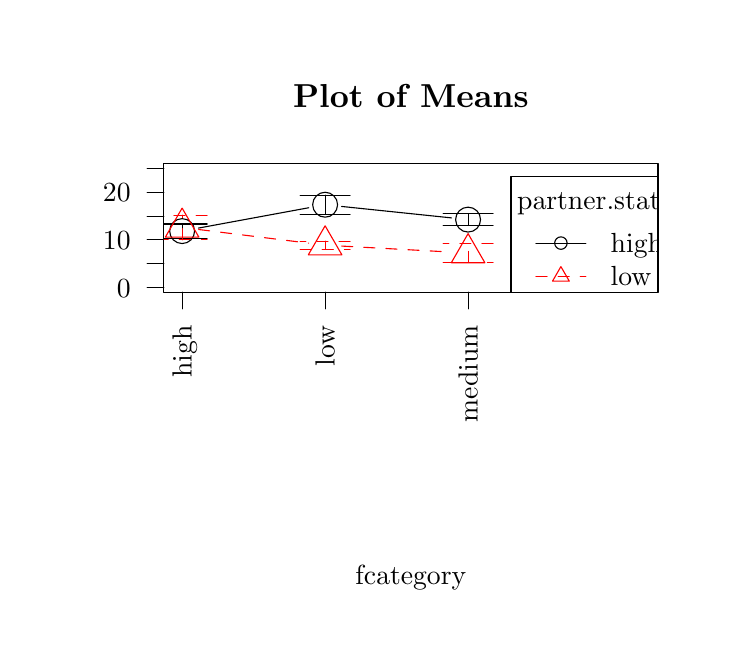
\begin{tikzpicture}[x=1pt,y=1pt]
\definecolor{fillColor}{RGB}{255,255,255}
\path[use as bounding box,fill=fillColor,fill opacity=0.00] (0,0) rectangle (252.94,216.81);
\begin{scope}
\path[clip] (  0.00,  0.00) rectangle (252.94,216.81);
\definecolor{drawColor}{RGB}{0,0,0}

\node[text=drawColor,anchor=base,inner sep=0pt, outer sep=0pt, scale=  1.20] at (138.47,188.07) {\bfseries Plot of Means};

\node[text=drawColor,anchor=base,inner sep=0pt, outer sep=0pt, scale=  1.00] at (138.47, 15.60) {fcategory};
\end{scope}
\begin{scope}
\path[clip] (  0.00,  0.00) rectangle (252.94,216.81);
\definecolor{drawColor}{RGB}{0,0,0}

\path[draw=drawColor,line width= 0.4pt,line join=round,line cap=round] ( 49.20,121.20) --
	(227.75,121.20) --
	(227.75,167.61) --
	( 49.20,167.61) --
	( 49.20,121.20);

\path[draw=drawColor,line width= 0.4pt,line join=round,line cap=round] ( 49.20,122.92) -- ( 49.20,165.89);

\path[draw=drawColor,line width= 0.4pt,line join=round,line cap=round] ( 49.20,122.92) -- ( 43.20,122.92);

\path[draw=drawColor,line width= 0.4pt,line join=round,line cap=round] ( 49.20,131.51) -- ( 43.20,131.51);

\path[draw=drawColor,line width= 0.4pt,line join=round,line cap=round] ( 49.20,140.11) -- ( 43.20,140.11);

\path[draw=drawColor,line width= 0.4pt,line join=round,line cap=round] ( 49.20,148.70) -- ( 43.20,148.70);

\path[draw=drawColor,line width= 0.4pt,line join=round,line cap=round] ( 49.20,157.30) -- ( 43.20,157.30);

\path[draw=drawColor,line width= 0.4pt,line join=round,line cap=round] ( 49.20,165.89) -- ( 43.20,165.89);

\node[text=drawColor,anchor=base east,inner sep=0pt, outer sep=0pt, scale=  1.00] at ( 37.20,119.48) {0};

\node[text=drawColor,anchor=base east,inner sep=0pt, outer sep=0pt, scale=  1.00] at ( 37.20,136.66) {10};

\node[text=drawColor,anchor=base east,inner sep=0pt, outer sep=0pt, scale=  1.00] at ( 37.20,153.85) {20};

\path[draw=drawColor,line width= 0.4pt,line join=round,line cap=round] ( 55.81,121.20) -- (159.14,121.20);

\path[draw=drawColor,line width= 0.4pt,line join=round,line cap=round] ( 55.81,121.20) -- ( 55.81,115.20);

\path[draw=drawColor,line width= 0.4pt,line join=round,line cap=round] (107.48,121.20) -- (107.48,115.20);

\path[draw=drawColor,line width= 0.4pt,line join=round,line cap=round] (159.14,121.20) -- (159.14,115.20);

\node[text=drawColor,rotate= 90.00,anchor=base east,inner sep=0pt, outer sep=0pt, scale=  1.00] at ( 59.26,109.20) {high};

\node[text=drawColor,rotate= 90.00,anchor=base east,inner sep=0pt, outer sep=0pt, scale=  1.00] at (110.92,109.20) {low};

\node[text=drawColor,rotate= 90.00,anchor=base east,inner sep=0pt, outer sep=0pt, scale=  1.00] at (162.58,109.20) {medium};
\end{scope}
\begin{scope}
\path[clip] ( 49.20,121.20) rectangle (227.75,167.61);
\definecolor{drawColor}{RGB}{0,0,0}

\path[draw=drawColor,line width= 0.4pt,line join=round,line cap=round] ( 61.71,144.39) -- (101.57,151.74);

\path[draw=drawColor,line width= 0.4pt,line join=round,line cap=round] (113.44,152.21) -- (153.17,148.07);

\path[draw=drawColor,line width= 0.4pt,line join=round,line cap=round] ( 55.81,143.30) circle (  4.50);

\path[draw=drawColor,line width= 0.4pt,line join=round,line cap=round] (107.48,152.83) circle (  4.50);

\path[draw=drawColor,line width= 0.4pt,line join=round,line cap=round] (159.14,147.45) circle (  4.50);

\path[draw=drawColor,line width= 0.4pt,line join=round,line cap=round] ( 55.81,140.74) -- ( 55.81,145.86);

\path[draw=drawColor,line width= 0.4pt,line join=round,line cap=round] ( 46.78,140.74) --
	( 55.81,140.74) --
	( 64.85,140.74);

\path[draw=drawColor,line width= 0.4pt,line join=round,line cap=round] ( 64.85,145.86) --
	( 55.81,145.86) --
	( 46.78,145.86);

\path[draw=drawColor,line width= 0.4pt,line join=round,line cap=round] (107.48,149.36) -- (107.48,156.29);

\path[draw=drawColor,line width= 0.4pt,line join=round,line cap=round] ( 98.44,149.36) --
	(107.48,149.36) --
	(116.51,149.36);

\path[draw=drawColor,line width= 0.4pt,line join=round,line cap=round] (116.51,156.29) --
	(107.48,156.29) --
	( 98.44,156.29);

\path[draw=drawColor,line width= 0.4pt,line join=round,line cap=round] (159.14,145.40) -- (159.14,149.50);

\path[draw=drawColor,line width= 0.4pt,line join=round,line cap=round] (150.10,145.40) --
	(159.14,145.40) --
	(168.17,145.40);

\path[draw=drawColor,line width= 0.4pt,line join=round,line cap=round] (168.17,149.50) --
	(159.14,149.50) --
	(150.10,149.50);
\definecolor{drawColor}{RGB}{255,0,0}

\path[draw=drawColor,line width= 0.4pt,dash pattern=on 4pt off 4pt ,line join=round,line cap=round] ( 61.77,143.88) -- (101.52,138.95);

\path[draw=drawColor,line width= 0.4pt,dash pattern=on 4pt off 4pt ,line join=round,line cap=round] (113.47,137.89) -- (153.15,135.71);

\path[draw=drawColor,line width= 0.4pt,line join=round,line cap=round] ( 55.81,151.62) --
	( 61.87,141.12) --
	( 49.75,141.12) --
	( 55.81,151.62);

\path[draw=drawColor,line width= 0.4pt,line join=round,line cap=round] (107.48,145.22) --
	(113.54,134.72) --
	(101.41,134.72) --
	(107.48,145.22);

\path[draw=drawColor,line width= 0.4pt,line join=round,line cap=round] (159.14,142.38) --
	(165.20,131.88) --
	(153.08,131.88) --
	(159.14,142.38);

\path[draw=drawColor,line width= 0.4pt,dash pattern=on 4pt off 4pt ,line join=round,line cap=round] ( 55.81,140.15) -- ( 55.81,149.08);

\path[draw=drawColor,line width= 0.4pt,dash pattern=on 4pt off 4pt ,line join=round,line cap=round] ( 46.78,140.15) --
	( 55.81,140.15) --
	( 64.85,140.15);

\path[draw=drawColor,line width= 0.4pt,dash pattern=on 4pt off 4pt ,line join=round,line cap=round] ( 64.85,149.08) --
	( 55.81,149.08) --
	( 46.78,149.08);

\path[draw=drawColor,line width= 0.4pt,dash pattern=on 4pt off 4pt ,line join=round,line cap=round] (107.48,136.78) -- (107.48,139.65);

\path[draw=drawColor,line width= 0.4pt,dash pattern=on 4pt off 4pt ,line join=round,line cap=round] ( 98.44,136.78) --
	(107.48,136.78) --
	(116.51,136.78);

\path[draw=drawColor,line width= 0.4pt,dash pattern=on 4pt off 4pt ,line join=round,line cap=round] (116.51,139.65) --
	(107.48,139.65) --
	( 98.44,139.65);

\path[draw=drawColor,line width= 0.4pt,dash pattern=on 4pt off 4pt ,line join=round,line cap=round] (159.14,131.99) -- (159.14,138.77);

\path[draw=drawColor,line width= 0.4pt,dash pattern=on 4pt off 4pt ,line join=round,line cap=round] (150.10,131.99) --
	(159.14,131.99) --
	(168.17,131.99);

\path[draw=drawColor,line width= 0.4pt,dash pattern=on 4pt off 4pt ,line join=round,line cap=round] (168.17,138.77) --
	(159.14,138.77) --
	(150.10,138.77);
\definecolor{drawColor}{RGB}{0,0,0}

\path[draw=drawColor,line width= 0.4pt,line join=round,line cap=round] (174.64,162.97) rectangle (240.40,114.97);

\path[draw=drawColor,line width= 0.4pt,line join=round,line cap=round] (183.68,138.97) -- (201.68,138.97);
\definecolor{drawColor}{RGB}{255,0,0}

\path[draw=drawColor,line width= 0.4pt,dash pattern=on 4pt off 4pt ,line join=round,line cap=round] (183.68,126.97) -- (201.68,126.97);
\definecolor{drawColor}{RGB}{0,0,0}

\path[draw=drawColor,line width= 0.4pt,line join=round,line cap=round] (192.68,138.97) circle (  2.25);
\definecolor{drawColor}{RGB}{255,0,0}

\path[draw=drawColor,line width= 0.4pt,line join=round,line cap=round] (192.68,130.47) --
	(195.71,125.22) --
	(189.65,125.22) --
	(192.68,130.47);
\definecolor{drawColor}{RGB}{0,0,0}

\node[text=drawColor,anchor=base,inner sep=0pt, outer sep=0pt, scale=  1.00] at (207.52,150.97) {partner.status};

\node[text=drawColor,anchor=base west,inner sep=0pt, outer sep=0pt, scale=  1.00] at (210.68,135.53) {high};

\node[text=drawColor,anchor=base west,inner sep=0pt, outer sep=0pt, scale=  1.00] at (210.68,123.53) {low};
\end{scope}
\end{tikzpicture}
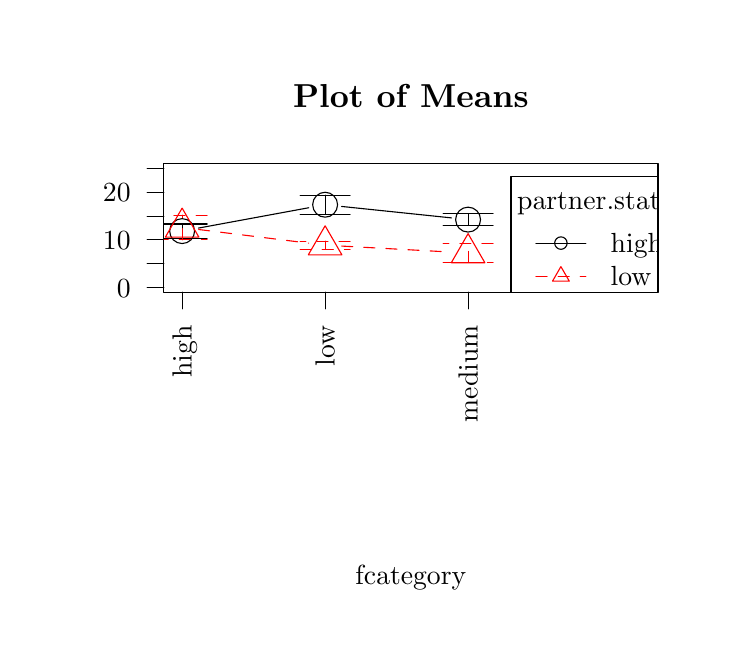
\begin{tikzpicture}[x=1pt,y=1pt]
\definecolor{fillColor}{RGB}{255,255,255}
\path[use as bounding box,fill=fillColor,fill opacity=0.00] (0,0) rectangle (252.94,216.81);
\begin{scope}
\path[clip] (  0.00,  0.00) rectangle (252.94,216.81);
\definecolor{drawColor}{RGB}{0,0,0}

\node[text=drawColor,anchor=base,inner sep=0pt, outer sep=0pt, scale=  1.20] at (138.47,188.07) {\bfseries Plot of Means};

\node[text=drawColor,anchor=base,inner sep=0pt, outer sep=0pt, scale=  1.00] at (138.47, 15.60) {fcategory};
\end{scope}
\begin{scope}
\path[clip] (  0.00,  0.00) rectangle (252.94,216.81);
\definecolor{drawColor}{RGB}{0,0,0}

\path[draw=drawColor,line width= 0.4pt,line join=round,line cap=round] ( 49.20,121.20) --
	(227.75,121.20) --
	(227.75,167.61) --
	( 49.20,167.61) --
	( 49.20,121.20);

\path[draw=drawColor,line width= 0.4pt,line join=round,line cap=round] ( 49.20,122.92) -- ( 49.20,165.89);

\path[draw=drawColor,line width= 0.4pt,line join=round,line cap=round] ( 49.20,122.92) -- ( 43.20,122.92);

\path[draw=drawColor,line width= 0.4pt,line join=round,line cap=round] ( 49.20,131.51) -- ( 43.20,131.51);

\path[draw=drawColor,line width= 0.4pt,line join=round,line cap=round] ( 49.20,140.11) -- ( 43.20,140.11);

\path[draw=drawColor,line width= 0.4pt,line join=round,line cap=round] ( 49.20,148.70) -- ( 43.20,148.70);

\path[draw=drawColor,line width= 0.4pt,line join=round,line cap=round] ( 49.20,157.30) -- ( 43.20,157.30);

\path[draw=drawColor,line width= 0.4pt,line join=round,line cap=round] ( 49.20,165.89) -- ( 43.20,165.89);

\node[text=drawColor,anchor=base east,inner sep=0pt, outer sep=0pt, scale=  1.00] at ( 37.20,119.48) {0};

\node[text=drawColor,anchor=base east,inner sep=0pt, outer sep=0pt, scale=  1.00] at ( 37.20,136.66) {10};

\node[text=drawColor,anchor=base east,inner sep=0pt, outer sep=0pt, scale=  1.00] at ( 37.20,153.85) {20};

\path[draw=drawColor,line width= 0.4pt,line join=round,line cap=round] ( 55.81,121.20) -- (159.14,121.20);

\path[draw=drawColor,line width= 0.4pt,line join=round,line cap=round] ( 55.81,121.20) -- ( 55.81,115.20);

\path[draw=drawColor,line width= 0.4pt,line join=round,line cap=round] (107.48,121.20) -- (107.48,115.20);

\path[draw=drawColor,line width= 0.4pt,line join=round,line cap=round] (159.14,121.20) -- (159.14,115.20);

\node[text=drawColor,rotate= 90.00,anchor=base east,inner sep=0pt, outer sep=0pt, scale=  1.00] at ( 59.26,109.20) {high};

\node[text=drawColor,rotate= 90.00,anchor=base east,inner sep=0pt, outer sep=0pt, scale=  1.00] at (110.92,109.20) {low};

\node[text=drawColor,rotate= 90.00,anchor=base east,inner sep=0pt, outer sep=0pt, scale=  1.00] at (162.58,109.20) {medium};
\end{scope}
\begin{scope}
\path[clip] ( 49.20,121.20) rectangle (227.75,167.61);
\definecolor{drawColor}{RGB}{0,0,0}

\path[draw=drawColor,line width= 0.4pt,line join=round,line cap=round] ( 61.71,144.39) -- (101.57,151.74);

\path[draw=drawColor,line width= 0.4pt,line join=round,line cap=round] (113.44,152.21) -- (153.17,148.07);

\path[draw=drawColor,line width= 0.4pt,line join=round,line cap=round] ( 55.81,143.30) circle (  4.50);

\path[draw=drawColor,line width= 0.4pt,line join=round,line cap=round] (107.48,152.83) circle (  4.50);

\path[draw=drawColor,line width= 0.4pt,line join=round,line cap=round] (159.14,147.45) circle (  4.50);

\path[draw=drawColor,line width= 0.4pt,line join=round,line cap=round] ( 55.81,140.74) -- ( 55.81,145.86);

\path[draw=drawColor,line width= 0.4pt,line join=round,line cap=round] ( 46.78,140.74) --
	( 55.81,140.74) --
	( 64.85,140.74);

\path[draw=drawColor,line width= 0.4pt,line join=round,line cap=round] ( 64.85,145.86) --
	( 55.81,145.86) --
	( 46.78,145.86);

\path[draw=drawColor,line width= 0.4pt,line join=round,line cap=round] (107.48,149.36) -- (107.48,156.29);

\path[draw=drawColor,line width= 0.4pt,line join=round,line cap=round] ( 98.44,149.36) --
	(107.48,149.36) --
	(116.51,149.36);

\path[draw=drawColor,line width= 0.4pt,line join=round,line cap=round] (116.51,156.29) --
	(107.48,156.29) --
	( 98.44,156.29);

\path[draw=drawColor,line width= 0.4pt,line join=round,line cap=round] (159.14,145.40) -- (159.14,149.50);

\path[draw=drawColor,line width= 0.4pt,line join=round,line cap=round] (150.10,145.40) --
	(159.14,145.40) --
	(168.17,145.40);

\path[draw=drawColor,line width= 0.4pt,line join=round,line cap=round] (168.17,149.50) --
	(159.14,149.50) --
	(150.10,149.50);
\definecolor{drawColor}{RGB}{255,0,0}

\path[draw=drawColor,line width= 0.4pt,dash pattern=on 4pt off 4pt ,line join=round,line cap=round] ( 61.77,143.88) -- (101.52,138.95);

\path[draw=drawColor,line width= 0.4pt,dash pattern=on 4pt off 4pt ,line join=round,line cap=round] (113.47,137.89) -- (153.15,135.71);

\path[draw=drawColor,line width= 0.4pt,line join=round,line cap=round] ( 55.81,151.62) --
	( 61.87,141.12) --
	( 49.75,141.12) --
	( 55.81,151.62);

\path[draw=drawColor,line width= 0.4pt,line join=round,line cap=round] (107.48,145.22) --
	(113.54,134.72) --
	(101.41,134.72) --
	(107.48,145.22);

\path[draw=drawColor,line width= 0.4pt,line join=round,line cap=round] (159.14,142.38) --
	(165.20,131.88) --
	(153.08,131.88) --
	(159.14,142.38);

\path[draw=drawColor,line width= 0.4pt,dash pattern=on 4pt off 4pt ,line join=round,line cap=round] ( 55.81,140.15) -- ( 55.81,149.08);

\path[draw=drawColor,line width= 0.4pt,dash pattern=on 4pt off 4pt ,line join=round,line cap=round] ( 46.78,140.15) --
	( 55.81,140.15) --
	( 64.85,140.15);

\path[draw=drawColor,line width= 0.4pt,dash pattern=on 4pt off 4pt ,line join=round,line cap=round] ( 64.85,149.08) --
	( 55.81,149.08) --
	( 46.78,149.08);

\path[draw=drawColor,line width= 0.4pt,dash pattern=on 4pt off 4pt ,line join=round,line cap=round] (107.48,136.78) -- (107.48,139.65);

\path[draw=drawColor,line width= 0.4pt,dash pattern=on 4pt off 4pt ,line join=round,line cap=round] ( 98.44,136.78) --
	(107.48,136.78) --
	(116.51,136.78);

\path[draw=drawColor,line width= 0.4pt,dash pattern=on 4pt off 4pt ,line join=round,line cap=round] (116.51,139.65) --
	(107.48,139.65) --
	( 98.44,139.65);

\path[draw=drawColor,line width= 0.4pt,dash pattern=on 4pt off 4pt ,line join=round,line cap=round] (159.14,131.99) -- (159.14,138.77);

\path[draw=drawColor,line width= 0.4pt,dash pattern=on 4pt off 4pt ,line join=round,line cap=round] (150.10,131.99) --
	(159.14,131.99) --
	(168.17,131.99);

\path[draw=drawColor,line width= 0.4pt,dash pattern=on 4pt off 4pt ,line join=round,line cap=round] (168.17,138.77) --
	(159.14,138.77) --
	(150.10,138.77);
\definecolor{drawColor}{RGB}{0,0,0}

\path[draw=drawColor,line width= 0.4pt,line join=round,line cap=round] (174.64,162.97) rectangle (240.40,114.97);

\path[draw=drawColor,line width= 0.4pt,line join=round,line cap=round] (183.68,138.97) -- (201.68,138.97);
\definecolor{drawColor}{RGB}{255,0,0}

\path[draw=drawColor,line width= 0.4pt,dash pattern=on 4pt off 4pt ,line join=round,line cap=round] (183.68,126.97) -- (201.68,126.97);
\definecolor{drawColor}{RGB}{0,0,0}

\path[draw=drawColor,line width= 0.4pt,line join=round,line cap=round] (192.68,138.97) circle (  2.25);
\definecolor{drawColor}{RGB}{255,0,0}

\path[draw=drawColor,line width= 0.4pt,line join=round,line cap=round] (192.68,130.47) --
	(195.71,125.22) --
	(189.65,125.22) --
	(192.68,130.47);
\definecolor{drawColor}{RGB}{0,0,0}

\node[text=drawColor,anchor=base,inner sep=0pt, outer sep=0pt, scale=  1.00] at (207.52,150.97) {partner.status};

\node[text=drawColor,anchor=base west,inner sep=0pt, outer sep=0pt, scale=  1.00] at (210.68,135.53) {high};

\node[text=drawColor,anchor=base west,inner sep=0pt, outer sep=0pt, scale=  1.00] at (210.68,123.53) {low};
\end{scope}
\end{tikzpicture}
